\documentclass[../main.tex]{subfiles}
\setlength{\columnsep}{4pt}
\begin{document}
  \noindent{\textit{A huge segmented insect with slender legs, each ending in a sharp claw, emerges from the ground in a burst of rock and dirt. A though chitinous brown shell covers its entire body, and glistening black eyes stare out from above powerfull mandibles.}}

  \begin{table}[H]
    \centering
    \begin{tabular}{lp{12em}}
      & \textbf{Large Magical Beast} \\
      \textbf{Hit Dice:} & 2d10+12 (28 hp) \\
      \textbf{Initiative:} & +0 \\
      \textbf{Speed:} & 30 ft. (6 squares), burrow 20 ft. \\
      \textbf{Armor Class:} & 18 (–1 size, +9 natural), touch 9, flat-footed 18 \\
      \textbf{Base Attack/Grapple:} & +3/+12 \\
      \textbf{Attack:} & Bite +7 melee (2d6+7 plus 1d4 acid) \\
      \textbf{Full Attack:} & Bite +7 melee (2d6+7 plus 1d4 acid) \\
      \textbf{Space/Reach:} & 10 ft./5 ft. \\
      \textbf{Special Attacks:} & Improved grab, spit acid \\
      \textbf{Special Qualities:} & Darkvision 60 ft., low-light vision, tremorsense 60 ft. \\
      \textbf{Saves:} & Fort +6, Ref +3, Will +2 \\
      \textbf{Abilities:} & Str 21, Dex 10, Con 17, Int 1, Wis 13, Cha 6 \\
      \textbf{Skills:} & Climb +8, Listen +6, Spot +3 \\
      \textbf{Feats:} & Alertness, Toughness \\
      \textbf{Environment:} & Warm plains \\
      \textbf{Organization:} & Solitary or cluster (2–4) \\
      \textbf{Challenge Rating:} & 3 \\
      \textbf{Treasure:} & None \\
      \textbf{Alignment:} & Always neutral \\
      \textbf{Advancement:} & 4 HD (Large); 5–9 HD (Huge) \\
      \textbf{Level Adjustment:} & -- \\
    \end{tabular}
  \end{table}

  \noindent{The ankheg is a burrowing monster with a taste for fresh meat.}\\
  \indent{An ankheg has six legs, and some specimens are yellow rather than brown. It is about 10 fet long and weighs about 800 pounds.}\\
  \indent{An ankheg burrows with legs and mandibles. A burrowing ankheg usually does not make a usable tunnel, but can construct a tunnel; it burrows at half speed when it does so. It often digs a winding tunnel up to 40 feet below the surface in the rich soil of forests or farmlands. The tunnel is 5 feet tall and wide, and from 60 to 150 feet long ([1d10 + 5] x 10). The hollowed ends of the tunnen serve as temporary lairs for sleeping, eating, or hibernating.}\\
  \indent{An can eat decayed organic matter but prefers fresh meat. Though a hungry ankheg might kill a farmer, the creature is quite beneficial to farmland. Its tunnel system laces the soil with passages for air an water, while its wastes add rich nutrients.}

  \dndsection{COMBAT}
  \noindent{An ankheg usually lies 5 to 10 feet below the surface until its antennae detect the approach of prey. It then burrows up to attack. (Treat this as a charge, even though the ankheg does not need to move 10 feet before attacking.)}\\
  \indent{Clusters of ankhegs share the same territory but do not cooperate.}\\
  \indent{\textbf{Improved Grab (Ex):} To use this ability, an ankheg must hit with its bite attack. It can then attempt to start a grapple as a free action without provoking an attack of opportunity. If the ankheg is damaged after grabbing its prey, it retreats backward down its tunnel at its land speed (not its burrow speed), dragging the victim with it.}\\
  \indent{\textbf{Spit Acid (Ex):} 30-ft. line, once every 6 hours; damage 4d4 acid, Reflex DC 14 half. One such attack depletes the ankheg’s acid supply for 6 hours. It cannot spit acid or deal acid damage during this time. The save DC is Constitution-based.}\\
  \indent{An ankheg does not use this ability unless it is desperate or frustrated. It most often spits acid when reduced to fewer than half its full normal hit points or when it has not successfully grabbed an opponent.}

  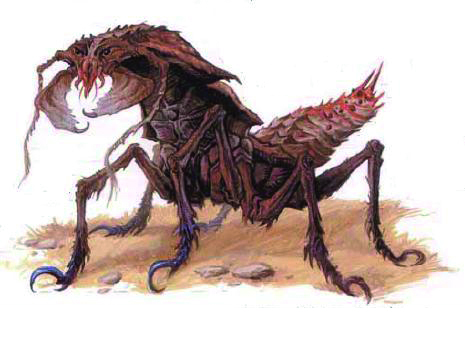
\includegraphics[width=\columnwidth]{Ankheg}

\end{document}
